In order to address the problem raised by Herley, we shall define how to
distinguish between a secure and an insecure system.  While most of the
literature have correlated the problem of in-security
to the maliciousness of agents interacting with the system, we show that
security doesn't seem to stem from a malicious nature but, rather, insecurity
raises from the lack of well-defined security requirements for the development
process of a system. We argue that the high number of security vulnerability
reported today are simply the realization of potential system configurations,
which deviate from the nominal behavior because the \emph{intended (or
nominal) behavior} of the system is not precisely defined in the specification
at the very early stages of the engineering process.   

\subsection{A Reference Model for Cybersecurity Engineering}\label{sec:vmodel}
A reference engineering process (so called, system security lifecycle of a
product) is described, in Section~\ref{sec:engineering}.  For the sake of
simplicity, we now give an high-level overview of a reference engineering model
focusing on the first three stages of the, so called, engineering V-Model. Our
definition is partial and we only use it  to
better present the theory.

The development process of a new product (a CPS in our case) 
should follow an engineering model. Our reference engineering process 
(inspired by the waterfall V-Model), as depicted in
Figure~\ref{fig:simplifiedvmodel}, is structured as the following ordered list
of abstraction refinement steps.
\begin{enumerate}
	\item The process starts with the definition of a \emph{specification}
		where the general requirements of the CPS are defined (e.g.
		functional, physical, network, and design).  As an example, an
		RFC of a communication or security protocol can be considered
		as the result of this first phase (e.g. see
		RFC-1\autocite{rfc1}.  In this first phase, we consider the
		architectural aspects of a CPS such as the draft physical and
		functional architectures.
	\item The process then continues with the definition of a design where
		the requirements of the previous phase holds; structuring the
		physical architecture along with its logic (e.g. the physical-layer encoding of the
		information), and the functional architectures and its logic (e.g. the protocol
		logic of communication over a number of potential sessions).
	\item Finally, the design is implemented as hardware (HW) for the physical architecture
		and software (SW) for the functional architecture.
\end{enumerate}

\begin{figure}[t]
	\centering
	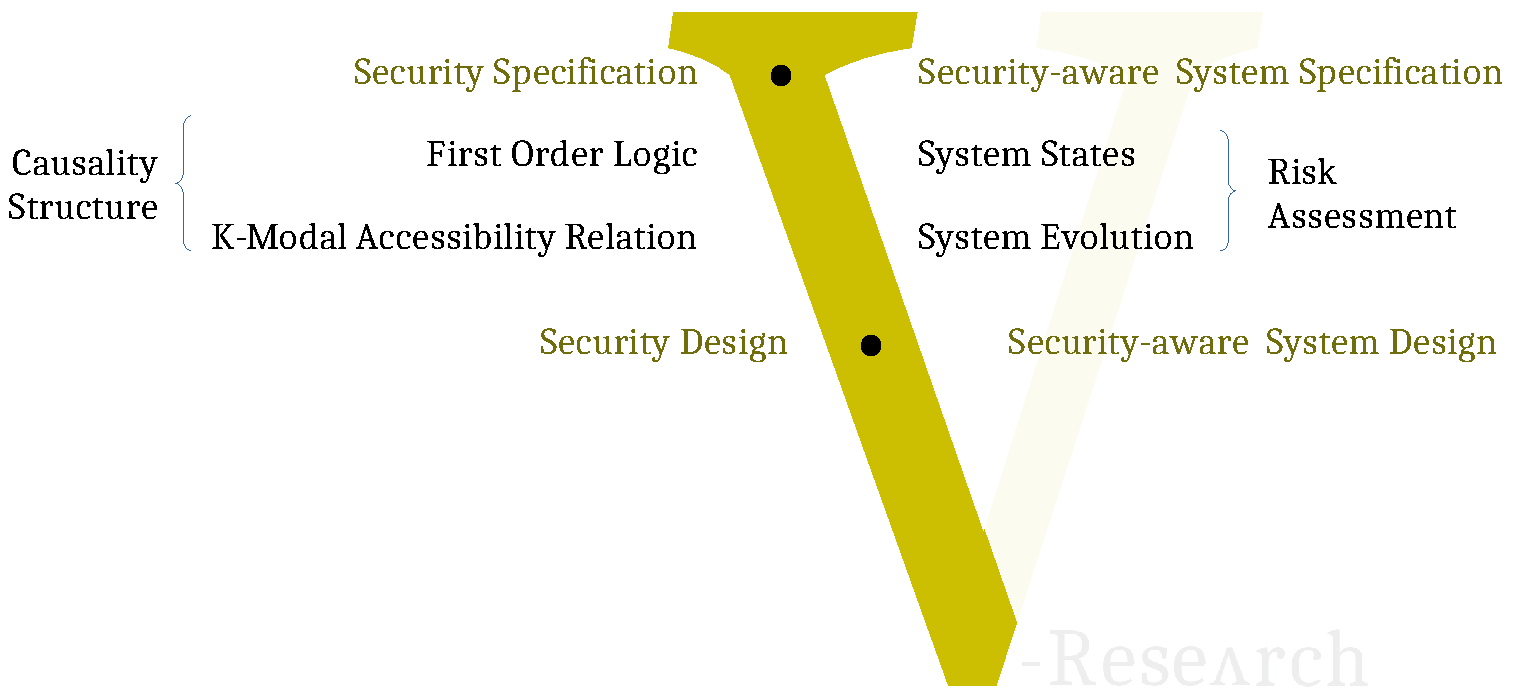
\includegraphics[width=\textwidth]{vmodel.pdf}
	\caption{Cybersecurity Engineering Life-cycle}
	\label{fig:simplifiedvmodel}
\end{figure}

Given that we apply our theory to \emph{systems engineering} and that
the two foundational processes (exploitation and hacking) are based on the
concept of a system, we shall begin by defining what a system is, in its
abstract form.

\subsection{Abstract System}\label{sec:systemstate}
The ISO/IEC/IEEE 15288:2015 (System Life Cycle Processes) provides a definition
of system as ``A combination of interacting elements organized to achieve one
or more stated purposes.''\autocite{ISO201515288}.  Therefore, a system can be
considered as a single agent where its interacting elements are the
constituents of the agent itself. For the sake of simplicity we first define a
system as an agent and then extend the definition to a ``combination of
interacting'' agents.  

There is no agreement between the research communities (e.g.
Multi-Agent-System, Epistemic Logic) on which are the constituent of an agent
as a system. However, the same ideas revolved around for thousands of years.
Some relevant examples for our objective are the following.
\begin{itemize}
	\item In \autocite{Hintikka1962knowledge}, Hintikka describes the
		difference between Knowledge and Belief (as epistemological
		concepts), and the whole Doxastic logic defines in details how
		Beliefs can be formalized.
	\item In \autocite{Hintikka1993Information}, Hintikka describes the concept
		of Information and the difference with Knowledge and Belief.
	%\item In \autocite{Empiricus1990Pyrrhonism}, the author states: ``The
	%	logical criterion also may be used in three senses -- of the
	%	agent, or the instrument, or the ``according to what''; the
	%	agent, for instance, may be a man, the instrument either sense
	%	perception or intelligence, and the ``according to what'' the
	%	application of the impression ``according to'' which the man
	%	proceeds to judge by means of one of the aforesaid
	%	instruments.'' 
	\item In \autocite{Santaca2016abf}, the authors defines an agent as a
		tuple of Assertions, Beliefs, and Facts.
\end{itemize}

\paragraph{Methodology}
The concept of Knowledge \autocite{Hintikka1962knowledge} (from an
epistemological point of view) can be defined as the way to get to the Truth.
Anything that is known is considered true\footnote{It is also
believed that Knowledge, defined as we did, is in-apprehensible \autocite{Empiricus1990Pyrrhonism}, but this shouldn't be an issue since it is a common problem to every scientific search}
In contrast, Beliefs \autocite{Hintikka1962knowledge} are potentially true and
leads to new hypothesis. Due to the
structure of deductive reasoning we can only start from unproven hypothesis and test the
deductive conclusions on the reality. Therefore, whatever a scientific-security-theory may be,
it can only be defined starting from hypotheses.  A sound reasoning should lead to
conclusion that shall be tested on a real system. Therefore, only at the end of
the reasoning we will be able to test, and judge, the quality of the theory
itself. The identification of hypotheses should start from probably true
beliefs (e.g. from Information \autocite{Hintikka1993Information}), and then from the state of the art.

For our argument, 
as in \autocite{Santaca2016abf}, an agent is composed by its knowledge, beliefs, and the information or assertions
it provides; where knowledge is defined, as in \autocite{Steup2020epistemology}, as
a set of proposition known by an agent, such that: (i) knowledge requires belief,
(ii) knowledge require truth, (iii) knowledge must be \emph{properly justified}, and
the only objective of Information is to exchange beliefs between agents.
As defined in \autocite{Hintikka1993Information}, ``Information is specified by specifying
which alternatives concerning the reality it admits and which alternatives
excludes''. This means that if we consider a propositional
variable (which admits the two alternatives True/False) its information is
defined as Believed to be True/False and not Believed to be the opposite. 
Due to the definition of Information and then with its relation to the probabilistic
correlation to truth/reality, we consider
information in relation with an agent's beliefs. Similarly, we consider
beliefs to define the actual behavior of an agent or a system. On the 
contrary, this view is not considered in most (if not all) the approaches to formal protocol verification
in the symbolic model. In fact, the security reasoning is usually applied to a representation/abstraction
of a protocol that only considers knowledge and transfer of knowledge (i.e.
if an agent sends a message, the recipient knows that message). However,
we believe that the security of a system is tightly related to the differences between
the nominal behavior and the actual (e.g. the implemented) one and only in the
nominal one (as hypothetical) one should consider agent's knowledge.

\begin{definition}{\bf System State and State-Space --}\label{def:system}
	The state of a system (or a sub-system or an agent) $s$ is defined as the tuple 
	$s=\langle\rcc(\knowledgeRegion,\beliefRegion),\rcc(\knowledgeRegion,\informationRegion),\rcc(\beliefRegion,\informationRegion)\rangle$,
	where $\knowledgeRegion,\beliefRegion,\informationRegion$ are Regions
	of Knowledge, Beliefs, and Information respectively, and $\rcc$ is a
	specific relation between Regions.  The
	state-space of a system is then defined by the different $\rcc$
	relations between the three pairs of Regions defining the system and
	all the sub-systems.
\end{definition}
Therefore, a system state space can be seen as a superposition of multiple agent states where knowledge,
beliefs, and information are related between each other (in a mereotopological
space) through all the admissible RCC relations. 
A \emph{system state} (as an instance of the system state space)
is a specific configuration of
the $\rcc$ relations between the three regions. Therefore, a collection of 
system states defines a collection of choices for those $\rcc$ relations.

% \item  ``normally concern the state or the history of the entire universe but only
% of some small part of
% it''.  
% \item  ``Information and probability are inversely related'', i.e. ``
% the more alternatives a proposition admits of, the more probable and the less
% informative it is, and vice versa''

\begin{figure}[t]
	\centering
	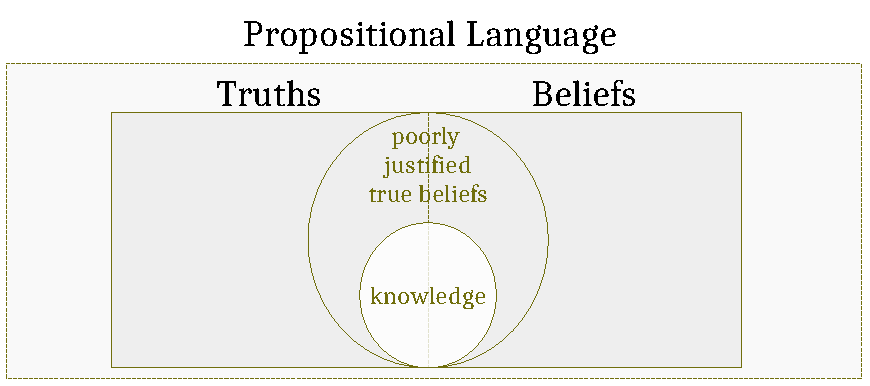
\includegraphics[width=.8\textwidth]{knowledge-belief.pdf}
	\caption{Informal representation of Knowledge and Belief}
	\label{fig:knowledge-belief}
\end{figure}

The difference between Knowledge and Belief is depicted in
Figure~\ref{fig:knowledge-belief} (see \autocite{wiki-knowledgebelief}).  However,
according to\autocite{Gettier2012knowledge},
Knowledge\footnote{``\emph{Theaetetus}: [\ldots] He said that knowledge was
true opinion accompanied by reason, but that unreasoning true opinion was
outside of the sphere of knowledge; and matters of which there is not a
rational explanation are unknowable -- yes, that is what he called them -- and
those of which there is are knowable. [\ldots] \emph{Socrates}: [\ldots] the
primary elements of which we and all else are composed admit of no rational
explanation; for each alone by itself can only be named, and no qualification
can be added, neither that it is nor that it is not, for that would at once be
adding to it existence or non-existence, whereas we must add nothing to it, if
we are to speak of that itself alone.  [\ldots]'' Plato -- Theaetetus 201
\autocite{Plato1914Plato}} as an epistemological concept is difficult to formally define. 
Similarly for the concept of information, Hintikka in \autocite{Hintikka1993Information}
states that ``A purely logical definition of information is impossible''.
In this work, however, we are not interested in how knowledge, information, or
belief can be precisely formalized from an epistemic standpoint.  We assume
that a semantic of a correct (i.e. commonly believed to be true) definition of epistemic knowledge exists, for
example the one given in\autocite{Hintikka1962knowledge} by Hintikka, and we
then define knowledge in terms of the Kripke structure defined in
Definition~\ref{def:modallogic}; similarly for Belief.

\begin{definition}{\bf Knowledge --}\label{def:knowledge}
Given an abstract collection of Agents $Ag$, and the modal operator
	$\knows{a}{}$ (where $a\in Ag$), Knowledge is defined as a region 
	of predicates known by an agent $\knowledge{a}=\bigcup_\Phi \knows{a}{\varphi}$ 
	(for all $\varphi\in\Phi$ where $\Phi$ is the collection of all the propositions known by $a$).
	Given a proposition $P$, we extend the semantics of the Causality structure with:
	\begin{enumerate}[noitemsep]
		\item[$(\interpretation16)$] $\world\models\knows{a}{P}$ iff
			$\world'\models P$ for all $\world'$ such that
			$\world\modalrelation\world'$.
	\end{enumerate}
\end{definition}

\begin{definition}{\bf Belief --}\label{def:belief}
	Given an abstract collection of Agents $Ag$, and the modal operator
	$\believe{a}{}$ (where $a\in Ag$), Belief is defined as a region 
	of predicates believed by an agent $\belief{a}=\bigcup_\Phi \believe{a}{\varphi}$
	(where $\Phi$ is the collection of all the propositions believed by $a$).
	Given a proposition $P$, we extend the semantics of the Causality structure with:
	\begin{enumerate}[noitemsep]
		\item[$(\interpretation17)$] $\world\models\believe{a}{P}$ iff
			$\world\models\neg\knows{a}{\neg P}$ (i.e. the agent $a$ considers $P$ possible) 
			and $\world'\models P$ for all
			$\world'$ such that $\world\modalrelation\world'$.
	\end{enumerate}
\end{definition}

\begin{definition}{\bf Information --}\label{def:information}
	Given an abstract collection of Agents $Ag$, and the modal operator
	$\informs{a}{}$ (where $a\in Ag$), Information is defined as a region 
	of beliefs asserted by an agents $a$.
	%and transferred from $a$ to $b$ ($a\rightarrow b$).
	$\information{a}=\bigcup_\Phi \informs{a}{}{\varphi}$
	(where $\Phi$ is the region of all the propositions believed and asserted by $a$).
	Given a proposition $P$, we extend the semantics of the Causality structure with:
	\begin{enumerate}[noitemsep]
		\item[$(\interpretation18)$] $\world\models\informs{a}{P}$ iff
			$\world\models\belief{a}{P}$ (i.e. the agent $a$ considers $P$ possible), 
			$\world\models\neg\belief{a}{\neg P}$%, 
			%and $\world'\models P$ for all
			%$\world'$ such that $\world\modalrelation\world'$.
	\end{enumerate}
\end{definition}

\subsection{Operational System}\label{sec:engsystemstate}
When dealing with a specification of a system (i.e. the design if the system
for a specific operation (as a generic operating/operational system),
considering abstract and general concepts such as knowledge, belief, or
information may result to be too abstract 
for the objectives of the overall engineering
process (e.g. verification and validation).
As an example, we are usually not
interested in information in abstract but to the transfer of that
information, which we call Assertions, made by a subset of agents. 
Therefore, we now define how we consider an agent for the engineering
of CPS.

\begin{enumerate}
	\item We consider Information only when the intention of exchanging 
		that Information is from a sender to 
		recipient is defined; and we call it \emph{Assertion}  
	\item Similarly, the portion of Beliefs we consider for system
		engineering is the one that builds (input) or describes
		(output) the behavior of an agent (strategy rules
		\footnote{``The logical structure of information is one of the
		most basic and one of the most basic and one of the simplest
		thing in the wide and wonderful world of logical analysis. This
		point can be put in a deeper perspective. A distinction
		[\ldots] ought to be made [--] between two kinds of rules (or
		principles) in any strategic activity like knowledge seeking.
		On the one hand you have the rules that define the game, e.g.
		how chessmen are moved on a board. The can be called
		\emph{definitory} rules.  They must be distinguished from rules
		[\ldots] that deal with what is better and what is worse in the
		game in question.  Definitory rules do not say anything about
		this subject. Rules which do can be called \emph{strategic
		rules}'' -- Hintikka in \autocite{Hintikka1993Information}}),
		and
	\item We consider a set of axiomatic \emph{Facts} (definitory rules\fixnote{mr}{facts are definitory rule, as they don't define how a real system is finally implemented (curently) but how it should, trugh a series of requirements which may not be respected, through insecurity, in the implemented system}) instead
		of considering the more general epistemic definition of
		Knowledge. Specifically, Facts describes:
		\begin{itemize}
			\item The functional architecture of each agents
			\item The physical/structural (HW/SW) architecture of each
				subsystem of agents and agent within a
				subsystem
			\item Assets and security properties
		\end{itemize}
\end{enumerate}
We give a graphical representation of (sub-)system and agent in Figure~\ref{fig:system-agent}.

We note here (and describe with more details afterwards in this paper) that the
data flow can be defined as a transfer of Beliefs through Assertions (i.e. the
Beliefs flow).

\begin{figure}[t]
	\centering
	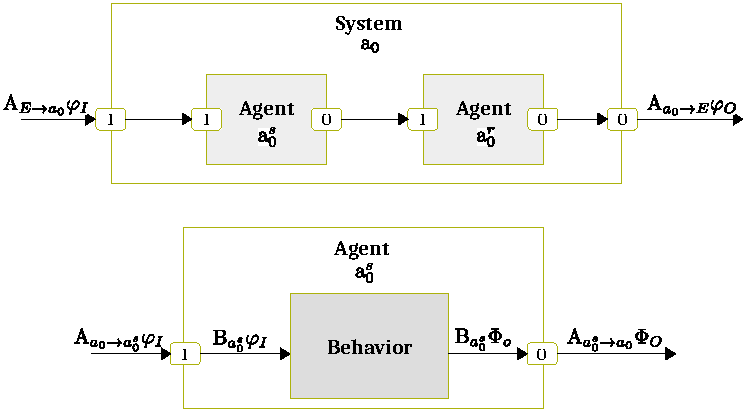
\includegraphics[width=.9\textwidth]{system-agent.pdf}
	\caption{Example of system and agent structure}
	\label{fig:system-agent}
\end{figure}

\begin{definition}{\bf Assertion -- }\label{def:assertion}
	An assertion is an intended transfer of beliefs between
	two agents $a$ and $b$ such that
	\begin{enumerate}[noitemsep]
		\item[$(\interpretation19)$] $\world\models\rassert{a}{b}{P}$ iff
			$\world\models\belief{a}{P}$, 
			$\world\models\neg\belief{a}{\neg P}$, 
			$\world'\models\rcc(\belief{a}{P},\belief{b}{P})$, 
			for all $\world'$ such that $\world\modalrelation\world'$.
	\end{enumerate}
\end{definition}

\begin{definition}{\bf Behavior -- }\label{def:behavior}
	The behavior of an agent is defined as the transformation process (e.g. defined as a
	protocol, or a functional architecture) that determines the
	output-beliefs based on input-beliefs and vice versa (where input-beliefs and
	output-beliefs are beliefs taken as input or output respectively).
	\begin{enumerate}[noitemsep]
		\item[$(\interpretation20)$] $\world\models\bigcup\behaviorRegion(\beliefRegion_I,\beliefRegion_O)$ and 
			$\world\models\beliefRegion_I\wedge\beliefRegion_O$,
		where $a$ is an agent, $\beliefRegion_I$ and $\beliefRegion_O$ are input and output-beliefs respectively.
	\end{enumerate}
\end{definition}

\begin{definition}{\bf Fact -- }\label{def:fact}
	Facts are defined as $\factRegion = \bigcup_\Phi \knows{a}{\varphi}$
	that predicate in a factive way, e.g.
	if $a$ knows that $P$ then $P$, and the region of facts is monotone (no revision).
	\begin{enumerate}[noitemsep]
		\item[$(\interpretation21)$] $\world\models\fact{a}{P}$ iff
			$\world \models \Box P$. 
	\end{enumerate}
\end{definition}

\begin{definition}{\bf Operational System State --}\label{def:opsystem}
	An operational system (or a sub-system) state is defined as the tuple
	$s=\langle\rcc(\factRegion,\behaviorRegion),\rcc(\factRegion,\assertionRegion),\rcc(\behaviorRegion,\assertionRegion)\rangle$,
	where $\assertionRegion,\behaviorRegion,\factRegion$, are regions of assertions, behavior (i.e. the beliefs generated by the behavior), and facts respectively.
\end{definition}

As already presented in \autocite{Santaca2016abf} it follows that, defining
a system (or an operational system) with a fixed number of regions, there exist
an upper-bound to the number of possible configuration of a system, defined by
the possible relations between the different regions.
For completeness, we report in the next paragraph 
the calculation done in \autocite{Santaca2016abf}.

\paragraph{Number of different configurations of a system}
The general formula to calculate the number of different types of agents is
$r^{\binom{n}{k}}$, where $r$ is the number of relations with arity $k$,
between $n$ different sets, where $r^e$ is the number of permutation of $r$
relations over $e$ elements with repetitions, with $e$ being the number of
$k$-ary combinations of $n$ sets, $\binom{n}{k}$.
In our case, $\binom{n}{k}=3$ since we consider $3$ sets
($\assertionRegion,\behaviorRegion,\factRegion$), and all the relations
considered in the RCC are binary.  Hence, using RCC5 (with five different
spatial relations) over three sets, we can theoretically define up to 125
different type of agents. However, only 54 of the 125 (as showed in
\cite{improvingRCC}) combinations are topologically correct with respect to
the definition of the relations of RCC5. Generalizing to all the RCCs:

\begin{itemize}%[nosep]
\item \emph{RCC3} --- theoretical: $3^3=27$,  correct: 15 
\item \emph{RCC5} --- theoretical: $5^3=125$, correct: 54
\item \emph{RCC8} --- theoretical: $8^3=512$, correct: 193
\end{itemize}

Hence, even if considering a different number of sets than the three
$\assertionRegion$, $\behaviorRegion$ and $\factRegion$ exponentially affects
the number of theoretical agents, the application of RCC downscales that number
of a factor that ranges from 1.8 to 2.5. In addition, using RCC5 we consider
3.6 times more (different) types of agents than RCC3, but using RCC8 would
allow us to consider 3.5 times more different agents.

In the quantitative evaluation of a single agent, depicted in Figure~\ref{fig:quantitative},
we argue that only 1 configuration represents the nominal (expected) behavior 
of the agent while the other configurations are either impossible to 
implement or diverge from the intended nominal behavior. We note 
that, the numbers reported here do not consider the details of the
engineering process and should be considered a limit of an abstract 
representation of the system. In Section~\ref{sec:engineering} we
detail this numeric evaluation to faithfully represent the
number of insecurity configurations, while in this section we consider
the general abstract definition given in Defintion~\ref{def:opsystem}.

\begin{figure}[t]
	\centering
	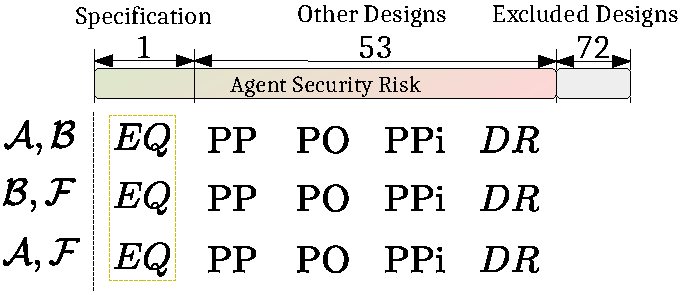
\includegraphics[width=.9\textwidth]{quantitative.pdf}
	\caption{Quantitative representation of the cybersecurity risk for a single agent}
	\label{fig:quantitative}
\end{figure}

As described beforehand in this section, the collection of Facts shall define
the functional and the physical architecture of an agent, but Assets and
security properties are defined as Facts, i.e. true. Given that understanding
why an Asset is considered as such by the user doesn't necessarily allow
us to better qualify an Asset, we consider the fact of ``being an asset'' as
a predicate of a component of a system. 

\begin{definition}{\bf Asset --}\label{def:asset}
For any agent $a\in Ag$ in a collection of Agents $Ag$, an agent is considered an asset iff 
	\begin{enumerate}[noitemsep]
		\item[$(\interpretation22)$] $\world\models\asset{a}$ iff
			$\world\models \Box\asset{a}$.
	\end{enumerate}
\end{definition}

The definition of the security properties is given in Section~\ref{sec:properties}

\subsection{Qualitative Evaluation of Agent Space in $\abftheory$}\label{sec:agentspace}
While a quantitative analysis reveals how many possible configurations of an
agent (i.e. a system) exist w.r.t. the $\abftheory$ theory (i.e. $54/125$ in RCC5), a
qualitative analysis of the different configurations describes
the configurations allowed by the $\abftheory$ theory, and how those configurations can be
categorized.  In Table~\ref{tab:5com} we provide the generic composition table
of RCC5 over 3 regions instantiated over $\abf$, which shows the whole state
space for a single agent. The color coding of the table represents the 
security risk related to a generic agent. 

As depicted in
Figure~\ref{fig:soundness}, the relation between Facts, and Assertions and Behavior
defines the soundness of the design (admissible configurations of Assertions,
Behaviors and, in turn, Beliefs) w.r.t. the specification (what the
specification mandates, such as by the nature of the physical/functional
architectural models). We categorize agents by first analyzing the relations
between each pair of Regions defining an agent (i.e. $\abf$), and then we
categorize the different agents as tuple of the three Regions.
For the sake of simplicity, soundness is opposed to non-soundness in the following, however,
with the RCC one should consider different ``degrees'' of non-soundness. For example,
in RCC5, if we consider EQ between two Regions as representing soundness, DR over the same Regions
represents non-soundness; while PP, PO, PPi represents the different degrees of non-soundness.
A similar argument can be done for completeness.
\fix{mr}{it's missing the relation with equivalence. missing parallelism with 
knowledge-belief/assertion (see slide v-research-demo)}
\begin{figure}[t]
	\centering
	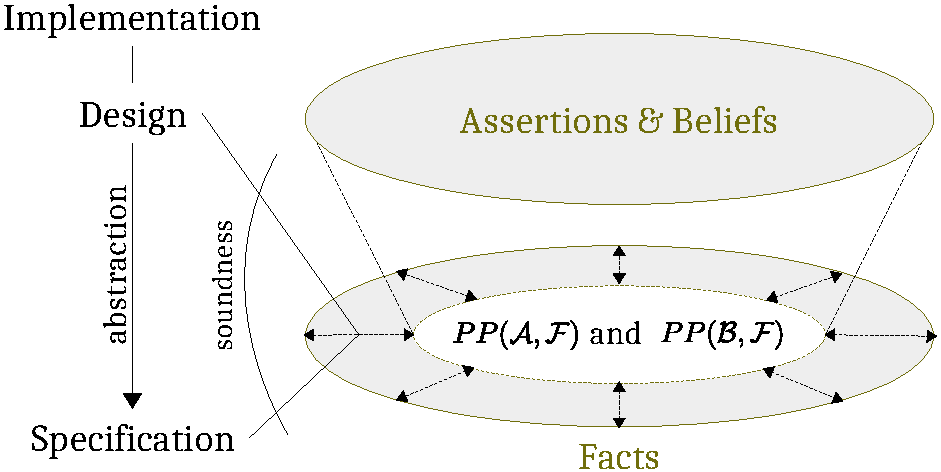
\includegraphics[width=.8\textwidth]{soundness.pdf}
	\caption{Example relation between Facts, and Assertions and Beliefs}
	\label{fig:soundness}
\end{figure}

\paragraph{\Rcc{$\assertionRegion$}{$\behaviorRegion$} -- Collaboration}
In order to reason on the relation between assertions and behavior we first
need to consider that, by definition, assertions are defined as transfer of
information between two agents, e.g., $a$ and $b$.  Therefore, as depicted in
Figure~\ref{fig:system-agent}, an agent has two main categories of assertions,
input and output assertions.  Given an agent $a$ and a collection of asserted
predicates $\Phi$, the Input assertions are those received by $a$ from an agent
$s$ acting as a sender, $\rassert{s}{a}{\Phi}$; similarly, output assertions
are sent from $a$ to a receiver $r$, $\rassert{a}{r}{\Phi}$. We shall consider
two pairs of regions\footnote{``I am not asserting, as Lotze did, that a relation between $X$ and $Y$
consists of a quality in $X$ and a quality in $Y$ -- a view which I regard as
quite indefensible. -- I assert that a relation $Z$ between $X$ and $Y$ involves
the existence in $X$ of the quality ``having the relation $Z$ to $Y$'' so that
a difference of relations always involves a difference in quality, and a
change of relations always involves a change of quality.'' --  Ellis J. McTaggart, The Unreality of Time\autocite{Mctaggart1908unreality}}: 
\begin{itemize}
	\item \Rcc{$\assertionRegion_{s\rightarrow a}$}{$\behaviorRegion$},
		where the relation between Input-assertions and behavior
		describes the soundness of the execution of the functional
		architecture w.r.t. input elicitation. With more details, the
		ideal specification of the functional architecture, along with
		the expected inputs, defines the functional behavior of an
		ideal system.  If all the inputs (Assertions) are correctly
		handled in the functional specification (behavior) the
		specification is complete. 

	\item \Rcc{$\assertionRegion_{a\rightarrow r}$}{$\behaviorRegion$},
		where the relation between behavior and outputs describes the
		completeness of the behavior defined in the specification
		w.r.t. the input elicitation.  With more details, if all the
		outputs (assertions) of the functional architecture can be
		produced, the functional architecture is complete.
\end{itemize}


\paragraph{\Rcc{$\assertionRegion$}{$\factRegion$} and \Rcc{$\behaviorRegion$}{$\factRegion$} -- Honesty and Competence}
While Assertions and Beliefs generated by the Behavior determines how a system should work, and the
relation between the two defines the quality (i.e. the completeness w.r.t the specification) of the agent, the relation of
Assertions and Behavior with Facts determines the quality with respect to the
nominal (specified) system.  Given that Facts defines what must be true in the
system, the relation of Assertions an Facts
determines the degree of quality between the information circulating in a
system (or within an agent) and reality\fixnote{mr}{assertions are reality
while facts are dogmatic assertions at specification level, i.e. requirements}.
Since the transfer of information through Assertions
generates Beliefs, a dishonest agent may circulate false information,
generating false Beliefs.  We note that it is often implied that the intention behind
circulating false information discerns a dishonest and an incompetent agent,
however, we consider honesty related to sharing truths\footnote{``[\ldots] truth
exists only in the good man, but the true in the bad man as well; for it is
possible for the bad man to utter something true.''
Sextus Empiricus, Outlines of Pyrrhonism, II-83\autocite{Empiricus1990Pyrrhonism}}.  The
relation between Beliefs and Facts determines the competence (on the subjects
defined by the Facts) of an agent (i.e. the more competent an agent is, the
more likely a Belief of that agent is true).

\subsubsection{$\abftheory$ Security Enumeration (SE)} The following security requirement for a CPS specification can be summarized:
\begin{enumerate}
	\item[SE-$1$] Proper interaction between correctly-behaving agents (in
		contrast with the ``Improper Interaction Between Multiple
		Correctly-Behaving Entities'' defined by the CWE--$435$ as one of the top ``view'' of the ``research concepts'' in
		\autocite{MITRE2020CWEresearch}) is defined as $\eq{\assertionRegion_a}{\behaviorRegion_a}$ for an agent $a$ while can be detailed as follows when multiple agents are considered.
	\begin{enumerate}
		\item[SE-$1.1$] The equality relation $\eq{\assertionRegion_{s\rightarrow a}}{\behaviorRegion_a}$
			describes the intended secure behavior as: the beliefs generated by the behavior of the functional architecture
			shall be complete w.r.t. the specified inputs of the agent. Therefore, \emph{the assertions received by an agent or a system
			shall be compliant with the expected inputs of the functional architecture}. For example, the inputs
			of the user of a SW must be sanitized to exclude deviations w.r.t. the expected inputs of the functions
			implemented in the SW. Another example is the type checking between allowed inputs and expected inputs.
		\item[SE-$1.2$] Similarly, the equality relation $\eq{\assertionRegion_{a\rightarrow r}}{\behaviorRegion_a}$ defines that
			the outputs of an agent $a$ shall be the outputs of the functional architecture.
	\end{enumerate}
	\item[SE-$2$]Sufficient Control Flow Management (in contrast with
		the ``Insufficient Control Flow Management'' defined by MITRE
		in the CWE--$691$ as one of the top ``view'' of the ``research
		concepts'' in\autocite{MITRE2020CWEresearch}) is defined as
		$\eq{\assertionRegion}{\factRegion}$.
	\item[SE-$3$] Correct Calculation (in contrast with the ``Improper
		Calculation'' defined by MITRE in the CWE--$682$ as one of the
		top ``view'' of the ``research concepts''
		in\autocite{MITRE2020CWEresearch}) is defined as
		$\eq{\behaviorRegion}{\factRegion}$.
\end{enumerate}

We are now in the position to define what a secure system is (with respect to the $\abftheory$-theory) 
and, based on that definition, what the security risk is and how to quantify it in a risk matrix.
\begin{definition}{\bf Security of a System or an Agent --}\label{def:security}
	A secure system is a system where SE-$1$, SE-$2$, and SE-$3$ holds for each 
	agent composing the system.
\end{definition}
The ISO 31000 consider risk as the ``effect of uncertainty on objectives'' and the refers
both of positive and negative consequences of uncertainty. Accordingly, we consider
risk as follows. 
\begin{definition}{\bf Risk --}
The whole space of potential designs of a specification with respect to the
$\abftheory$-theory.
\end{definition}
The definition of Risk leads to the risk matrix in Figure~\ref{fig:quantitative}, defined as follows.
\begin{definition}{\bf Risk Matrix --}
	The risk matrix is a function between the three relations 
	$s=\langle\rcc(\factRegion,\behaviorRegion),\rcc(\factRegion,\assertionRegion),\rcc(\behaviorRegion,\assertionRegion)\rangle$,
	where the maximum risk is defined by the $DR$ relation between the three groups of Regions, and the 
	minimum risk by the $EQ$ relation over the same Regions. In between the two extremes, the granularity
	of possible intermediate configuration is defined by the calculus used (RCC5 in our case).
\end{definition}
We note that often the risk matrix is defined by the relation between likelihood and impact which we
discuss in the next section.

\begin{table}[t]
\centering
\begin{adjustbox}{width=\textwidth}
\begin{tabular}{r||c|c|c|c|c} 
& \dr{$\assertionRegion$}{$\behaviorRegion$} & 
	\po{$\assertionRegion$}{$\behaviorRegion$}& 
	\pp{$\assertionRegion$}{$\behaviorRegion$} &
	\ppi{$\assertionRegion$}{$\behaviorRegion$} & 
	\eq{$\assertionRegion$}{$\behaviorRegion$} \\
\hline
\hline %dr
 \multirow{3}{*}{\dr{$\behaviorRegion$}{$\factRegion$}} & 
	\cellcolor{abfred} & %dr
	\cellcolor{abf-rg-1}\dr{$\assertionRegion$}{$\factRegion$} & %po
	\cellcolor{abf-rg-2}\multirow{3}{*}{\dr{$\assertionRegion$}{$\factRegion$}} & %pp
	\cellcolor{abf-rg-3} \dr{$\assertionRegion$}{$\factRegion$}& % ppi
	 \cellcolor{abf-rg-4} \\ % eq
& \cellcolor{abfred}\all{$\assertionRegion$}{$\factRegion$}& %dr
	\cellcolor{abf-rg-1}\po{$\assertionRegion$}{$\factRegion$} & %po
	\cellcolor{abf-rg-2}\dr{$\assertionRegion$}{$\factRegion$} & %pp
	\cellcolor{abf-rg-3}\po{$\assertionRegion$}{$\factRegion$} & %ppi
	\cellcolor{abf-rg-4}\dr{$\assertionRegion$}{$\factRegion$}\\ % e q
 & \cellcolor{abfred}& %dr
	\cellcolor{abf-rg-1}\pp{$\assertionRegion$}{$\factRegion$} & %po
	\cellcolor{abf-rg-2}  & %pp
	\cellcolor{abf-rg-3}\pp{$\assertionRegion$}{$\factRegion$} & %ppi
	\cellcolor{abf-rg-4} \\ %eq
\hline %po
 \multirow{3}{*}{\po{$\behaviorRegion$}{$\factRegion$}} &
	\cellcolor{abf-rg-1}\dr{$\assertionRegion$}{$\factRegion$} & %dr
	\cellcolor{abf-rg-2} & %po
	\cellcolor{abf-rg-3}\dr{$\assertionRegion$}{$\factRegion$} & %pp
	\cellcolor{abf-rg-4}\po{$\assertionRegion$}{$\factRegion$} & %ppi
	\cellcolor{abf-rg-5} \\ %eq
 & \cellcolor{abf-rg-1}\po{$\assertionRegion$}{$\factRegion$} & %dr
	\cellcolor{abf-rg-2} \all{$\assertionRegion$}{$\factRegion$} & %po 
	\cellcolor{abf-rg-3}\po{$\assertionRegion$}{$\factRegion$} & %pp
	\cellcolor{abf-rg-4}\ppi{$\assertionRegion$}{$\factRegion$} & %ppi
	\cellcolor{abf-rg-5} \po{$\assertionRegion$}{$\factRegion$}\\%eq
 & \cellcolor{abf-rg-1}\pp{$\assertionRegion$}{$\factRegion$} & %dr
	\cellcolor{abf-rg-2} &  %po
	\cellcolor{abf-rg-3}\pp{$\assertionRegion$}{$\factRegion$} & %pp
	\cellcolor{abf-rg-4}& %ppi
	\cellcolor{abf-rg-5}\\ %eq
\hline %pp
 \multirow{4}{*}{\pp{$\behaviorRegion$}{$\factRegion$}} &
	\cellcolor{abf-rg-2}\dr{$\assertionRegion$}{$\factRegion$} & 
	\cellcolor{abf-rg-3}&
	\cellcolor{abf-rg-4} & %pp
	\cellcolor{abf-rg-5}\po{$\assertionRegion$}{$\factRegion$} & %ppi
	\cellcolor{abf-rg-6}\\ %eq
 & \cellcolor{abf-rg-2}\po{$\assertionRegion$}{$\factRegion$} & 
	\cellcolor{abf-rg-3}\po{$\assertionRegion$}{$\factRegion$} & 
	\cellcolor{abf-rg-4}\pp{$\assertionRegion$}{$\factRegion$} & %pp
	\cellcolor{abf-rg-5}\eq{$\assertionRegion$}{$\factRegion$} & %ppi
	\cellcolor{abf-rg-6}\pp{$\assertionRegion$}{$\factRegion$} \\ %eq
 & \cellcolor{abf-rg-2}\pp{$\assertionRegion$}{$\factRegion$} & 
	\cellcolor{abf-rg-3}\pp{$\assertionRegion$}{$\factRegion$} & 
	\cellcolor{abf-rg-4} & %pp
	\cellcolor{abf-rg-5}\pp{$\assertionRegion$}{$\factRegion$} & %ppi
	\cellcolor{abf-rg-6} \\ %eq
 & \cellcolor{abf-rg-2}&
 	\cellcolor{abf-rg-3} & 
	\cellcolor{abf-rg-4}& %pp
	\cellcolor{abf-rg-5}\ppi{$\assertionRegion$}{$\factRegion$} & %ppi
	\cellcolor{abf-rg-6} \\ %eq
\hline %ppi
 \multirow{3}{*}{\ppi{$\behaviorRegion$}{$\factRegion$}} &
 	\cellcolor{abf-rg-3}\multirow{3}{*}{} &
 	\cellcolor{abf-rg-4}\dr{$\assertionRegion$}{$\factRegion$} &
 	\cellcolor{abf-rg-5}& %pp
 	\cellcolor{abf-rg-6}& %ppi
 	\cellcolor{abf-rg-7} \\ %eq
& \cellcolor{abf-rg-3}\dr{$\assertionRegion$}{$\factRegion$} &
 	\cellcolor{abf-rg-4}\po{$\assertionRegion$}{$\factRegion$} & 
 	\cellcolor{abf-rg-5}\all{$\assertionRegion$}{$\factRegion$}& %pp
 	\cellcolor{abf-rg-6}\ppi{$\assertionRegion$}{$\factRegion$}& %ppi
 	\cellcolor{abf-rg-7}\ppi{$\assertionRegion$}{$\factRegion$}\\ %eq
& \cellcolor{abf-rg-3} & 
	\cellcolor{abf-rg-4}\ppi{$\assertionRegion$}{$\factRegion$} & 
	\cellcolor{abf-rg-5} & %pp
	\cellcolor{abf-rg-6}& %ppi
	\cellcolor{abf-rg-7}\\ %eq
\hline %eq
	\eq{$\behaviorRegion$}{$\factRegion$} & 
	\cellcolor{abf-rg-4}\dr{$\assertionRegion$}{$\factRegion$} & 
	\cellcolor{abf-rg-5} \po{$\assertionRegion$}{$\factRegion$} & 
	\cellcolor{abf-rg-6}\pp{$\assertionRegion$}{$\factRegion$} & %pp
	\cellcolor{abf-rg-7} \ppi{$\assertionRegion$}{$\factRegion$} & %ppi 
	\cellcolor{abfgreen} \eq{$\assertionRegion$}{$\factRegion$}  %eq
\end{tabular}
\end{adjustbox}
\caption{RCC5 composition table over 3 regions. The results show that there
exist 54 possible relations and the coloring anticipates the ideal risk matrix
(green the secure state with low risk, red the high risk state, and a gradient
of medium risk states). 
\all{$\assertionRegion$}{$\factRegion$} = \{\dr{$\assertionRegion$}{$\factRegion$}, \po{$\assertionRegion$}{$\factRegion$}, \pp{$\assertionRegion$}{$\factRegion$}, \ppi{$\assertionRegion$}{$\factRegion$}, \eq{$\assertionRegion$}{$\factRegion$}\}
\label{tab:5com}}
\end{table}
